\documentclass[12pt]{article}
\usepackage[margin=4cm]{geometry} % Set page margins
\usepackage{graphicx} % Required for inserting images
\bibliographystyle{ieeetr}  % Specifies the IEEE Transactions reference style
\usepackage{subcaption} % Create subfigures under a single figure environment
\usepackage{wrapfig} % Allows text to wrap around figures
\usepackage{float} % Control figure and table placement (for [H] option)
\usepackage{slashbox} % Create diagonal slash tables (used for splitting cells)
% Mathematics and Theorem Environments
\usepackage{amsmath} % Provides enhanced math typesetting (equations, symbols)
\usepackage{amsfonts} % Additional fonts for math (e.g., Blackboard bold, Fraktur)
\usepackage{amsthm} % For defining theorem-like environments (theorems, propositions, definitions)
\newtheorem{definition}{Definition} % Define the environment for definitions
\newtheorem{proposition}{Proposition} % Define the environment for propositions
\usepackage{lineno} % For line numbers in the document
\usepackage{titlesec} % Control section title formatting
% Referencing and Hyperlinks
\usepackage{hyperref} % Create hyperlinks in the document (for references, citations, tables, etc.)
\usepackage{xcolor} % For coloring text
\usepackage[normalem]{ulem} % For strikethrough text
% \usepackage{multicol}

\title{The History Behind Leap Year}
\author{Mosharaf Hossain Apurbo(2105057)}
\date{\today}

\begin{document}

\sloppy 

\maketitle

\section{Introduction}

A leap year is a calendar year that contains an additional day compared to a commonyear\cite{meeus1991astronomical}. This article covers the development of the leap year system and its importance in keeping our calendar aligned with Earth’s revolution around the sun.

\section{History}
\textcolor{blue}{Did you know?} The Earth takes about 365 days to orbit the Sun, but it’s not exactly 365. In fact, it’s around \textcolor{red}{\sout{365}} \textcolor{green}{365.24}

    \subsection{Julian Calendar}
    Introduced by Julius Caesar (Figure \ref{fig:fig1}) in 45 BC, the “Julian Calendar” included a leap year every four years. This was necessary because the solar year is approximately 365.25 days long.

    \subsection{Gregorian Calendar}
     The modern leap year system was developed under Gregory XIII (Figure \ref{fig:fig2}) in 1582. In the “Gregorian Calendar”, leap years are introduced every four years, except years divisible by 100 but not divisible by 400.

    \begin{figure}[h]
        \centering
        \begin{subfigure}[b]{0.4\textwidth}
            \centering
            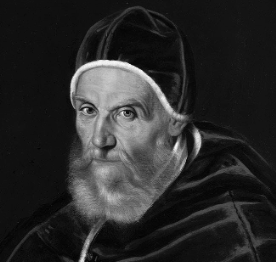
\includegraphics[width=\textwidth]{gregory.PNG} % Change to the actual filename
            \caption{Julius}
            \label{fig:fig1}
        \end{subfigure}
        \hspace{.1cm}
        \begin{subfigure}[b]{0.4\textwidth}
            \centering
            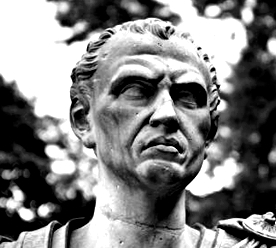
\includegraphics[width=\textwidth]{julius.jpg} % Change to the actual filename
            \caption{Gregory}
            \label{fig:fig2}
        \end{subfigure}
        \caption{Pioneers of Modern Calendars}
        \label{fig:calendars}
    \end{figure}



\section{Leap Year Rules}
 The rules for calculating a leap year can be summarized as:

    \begin{enumerate}
        \item \textbf{A year is a leap year if}:
        \begin{enumerate}
            \item It is divisible by 4 and not divisible by 100.
            \item Or it is divisible by 400.
        \end{enumerate}
        \item \textbf{A year is \textit{NOT} a leap year \underline{in all other cases}.}
    \end{enumerate}

    

\section{Leap Year Calculation Formula}
 The formula to determine if a year Y is a leap year (or not) is written below.

 $ \text{Leap Year} = 
\begin{cases}
\textbf{True,} & \text{if } (Y\: \% 4 = 0 \&\& Y \% 100 \neq 0 )\| Y \% 400 = 0 ) \\
\textbf{False,}  & \text{ } \text{otherwise}
\end{cases}$


Some examples of leap year calculations are shown in Table 1.
    \begin{table}[h]
    \centering
    \begin{tabular}{|c|c|c|c|c|}
        \hline
        Year & \multicolumn{3}{c|}{Divisible By} & Leap Year? \\
        \cline{2-4}
        & 4? & 100? & 400? & \\
        \hline
        1900 & Yes & Yes & No & No \\
        \hline
        2000 & Yes & Yes & Yes & Yes \\
        \hline
        2024 & Yes & No & No & Yes \\
        \hline
    \end{tabular}
    \caption{Leap Year Calculation Examples}
    \label{tab:leap-year-examples}
    \end{table}

 
\section{Importance}
The Earth takes approximately 365.24 days to complete one orbit around the sun. This discrepancy accumulates, and leap years help correct it. Without leap years, seasons would gradually drift over time.


\section*{Disclaimer}
 Thearticle is designed with the sole purpose of evaluating students’  \LaTeX 
 proficiency.


\bibliography{mybibfile}  % This assumes you have a BibTeX file named mybibfile.bib

\end{document}
